\documentclass{beamer}
\usepackage[framemethod=TikZ]{mdframed}
\usepackage[percent]{overpic}
\usepackage{graphicx}
\usepackage{color}
\usepackage{hyperref}
\usepackage{fancybox}
\usepackage{appendixnumberbeamer}

\usetheme[left,hideothersubsections,height=1.2cm,width=2.0cm]{UNLTheme}

\title[\textbf{Silicon Telescope}]{-- FPIX-Phase 2 Upgrade Meeting -- \\ \textbf{High-Precision Silicon Strip Telescope}}
\author{Caleb~Fangmeier}
\institute[UNL]{University of Nebraska - Lincoln}
\date{Sept 27, 2016}
\subject{High-Precision Silicon Strip Telescope}


\mdfsetup{skipabove=\topskip,skipbelow=\topskip}
\mdfdefinestyle{curvedtranslucent}{%
  outerlinewidth=0pt,innerlinewidth=0pt,
  outerlinecolor=gray,
  roundcorner=8pt,
  tikzsetting={fill=white,
               fill opacity=0.9},
  backgroundcolor=none
}
\newcommand{\checkedbox}{$\text{\rlap{$\checkmark$}}\square$}
\newcommand{\checkbox}{$\square$}

\begin{document}

\begin{frame}
  \titlepage
\end{frame}

\begin{frame}{Telescope Overview}
    \begin{figure}
    \centering
    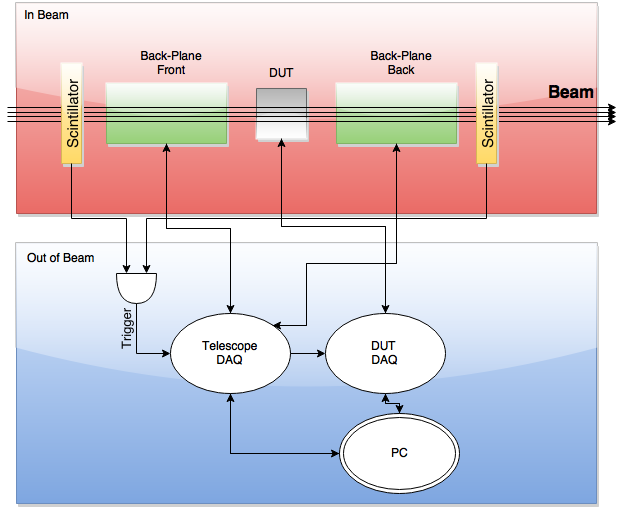
\includegraphics[width=0.9\textwidth]{figures/Telescope_Hierarchy}
    \end{figure}
\end{frame}

\section{Hardware}

\begin{frame}{Back-Plane Board (``Motherboard'')}
\vspace{-.75in}
\begin{figure}
    \begin{overpic}[height=2.0in, width=\textwidth]{figures/Half-Telescope-Full}
      \put(4,7){%
        \begin{minipage}[t]{0.90\textwidth}
          \begin{mdframed}[style=curvedtranslucent]
            \begin{columns}[t]
              \begin{column}{.02\textwidth}\end{column} %Spacer column
              \begin{column}{0.5\textwidth}
                \textbf{Features}
                \begin{itemize}
                  \itemsep0em 
                  \tiny
                  \item Each card can be used to measure either $x$ or $y$ track position
                  \item Configuration shown has alternating $x$ and $y$ measurements
                  \item Shared control signals for synchronous data taking
                  \item Individual output channels for fast readout
                  \item Fast readout is critical to minimize downtime
                \end{itemize}
              \end{column}
              \vrule{}
              \begin{column}{0.5\textwidth}
                \textbf{Components}
                \begin{itemize}
                  \itemsep0em 
                  \tiny
                  \item 4$\times$Sensor Cards, each with
                  \begin{itemize}
                    \itemsep0em 
                    \tiny
                    \item 1$\times$512-channel micro-strip sensor
                    \item 4$\times$APC-128
                    \item 4$\times$AD8138 buffer amplifiers
                    \item 4$\times V_{analog}$ trimmer potentiometers
                  \end{itemize}
                  \item 4$\times$RJ-45 Ports
                  \item 1$\times$40-Pin $0.1$in~Header
                \end{itemize}
              \end{column}
            \end{columns}
          \end{mdframed}
        \end{minipage}
        }
    \end{overpic}
\end{figure}
\end{frame}

\begin{frame}{Analog Pipeline Chip \-- 128}
\vspace{-.75in}
\begin{figure}
    \begin{overpic}[height=2.00in, width=\textwidth]{figures/APC128_Schematic}
      \put(4,3){%
        \begin{minipage}[t]{0.90\textwidth}
          \begin{mdframed}[style=curvedtranslucent]
            \tiny
            \begin{itemize}
            \itemsep0em 
              \item Developed for the tracker of the H1 detector at HERA
              \item Serializes the analog pulse-heights of 128 channels to dramatically reduce the number of required I/O lines
              \item Capable of sampling waveform data from of a strip sensor at upwards of 20MHz
              \item Features a very good signal-to-noise ratio of 40
              \item Low noise combined with inter-strip charge-sharing give each layer of the detector a measurement precision of $\approx\negthickspace1\mu$m
            \end{itemize}
          \end{mdframed}
        \end{minipage}
        }
    \end{overpic}
\end{figure}
\end{frame}

\begin{frame}{Data Acquisition (DAQ) Board}
\vspace{-.85in}
\begin{figure}
    \begin{overpic}[height=2.0in, width=\textwidth]{figures/DAQ_Board_Real.png}
      \put(4,7){%
        \begin{minipage}[t]{0.90\textwidth}
          \begin{mdframed}[style=curvedtranslucent]
            \begin{columns}[t]
              \begin{column}{.02\textwidth}\end{column} %Spacer column
              \begin{column}{0.50\textwidth}
                \textbf{Features}
                \tiny
                \begin{itemize}
                  \itemsep0em 
                  \item Generates the control signals needed by the APC-128s
                  \item 32 ADC Channels to read out all APC128s in parallel, minimizing dead time
                  \item FPGA Board with associated USB hardware enables high-speed communication with online software
                  \item Handles external triggering from a variety of sources via a translator mezzanine card
                \end{itemize}
              \end{column}
              \vrule{}
              \begin{column}{0.50\textwidth}
                \textbf{Components}
                \begin{itemize}
                  \itemsep0em 
                  \tiny
                  \item $1\times$\textbf{\textit{Opal Kelly} ZEM4310} with
                    \begin{itemize}
                      \itemsep0em 
                      \tiny
                      \item Cyclone IV FPGA
                      \item 128MB RAM
                      \item USB-3.0
                      \item $2\times$HSMC Connectors
                    \end{itemize}
                  \item $8\times$AD9219 40MHz/10 bit ADCs
                  \item $8\times$RJ-45 Ports
                  \item $2\times$40-Pin $0.1$in~Header
                  \item Bias-voltage control relay
                  \item On-board power regulation
                \end{itemize}
              \end{column}
            \end{columns}
          \end{mdframed}
        \end{minipage}
        }
    \end{overpic}

\end{figure}
\end{frame}

\section{Readout}

\begin{frame}{Readout: In-Beam}
\begin{figure}
\centering
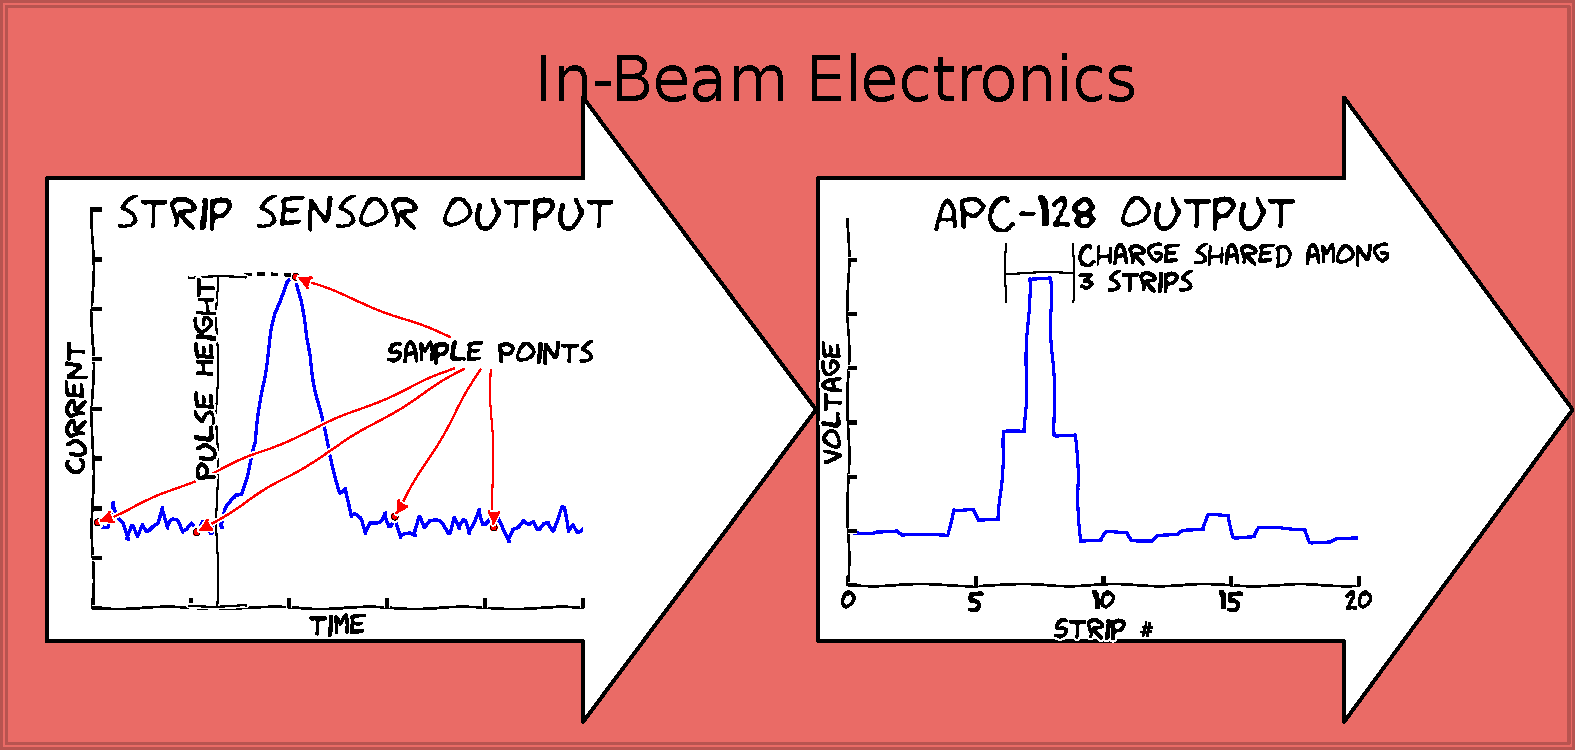
\includegraphics[width=\textwidth]{figures/B1}
\end{figure}
\end{frame}

\begin{frame}{Readout: DAQ Board}
\begin{figure}
\centering
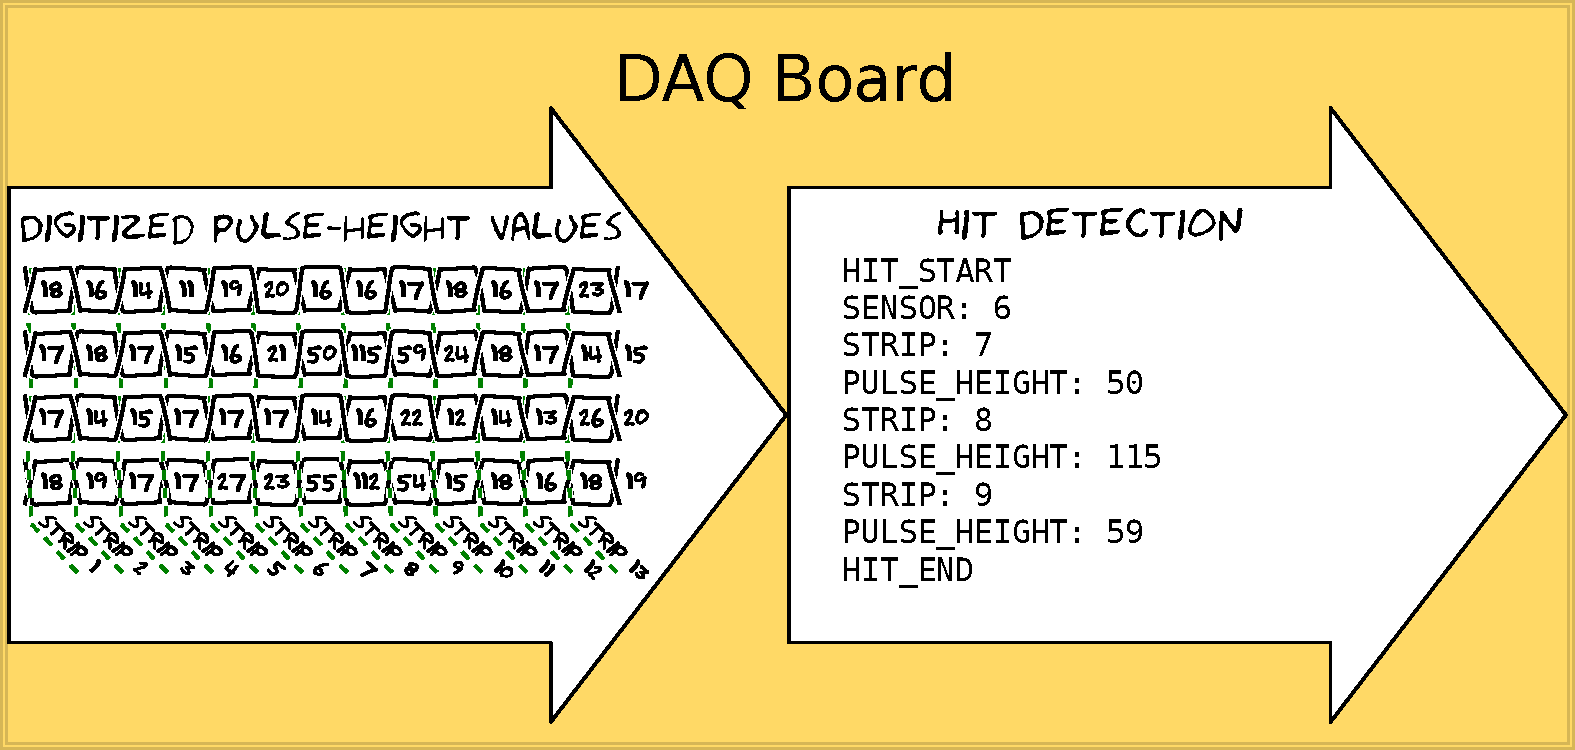
\includegraphics[width=\textwidth]{figures/B2}
\end{figure}
\end{frame}

\begin{frame}{Readout: PC}
\begin{figure}
\centering
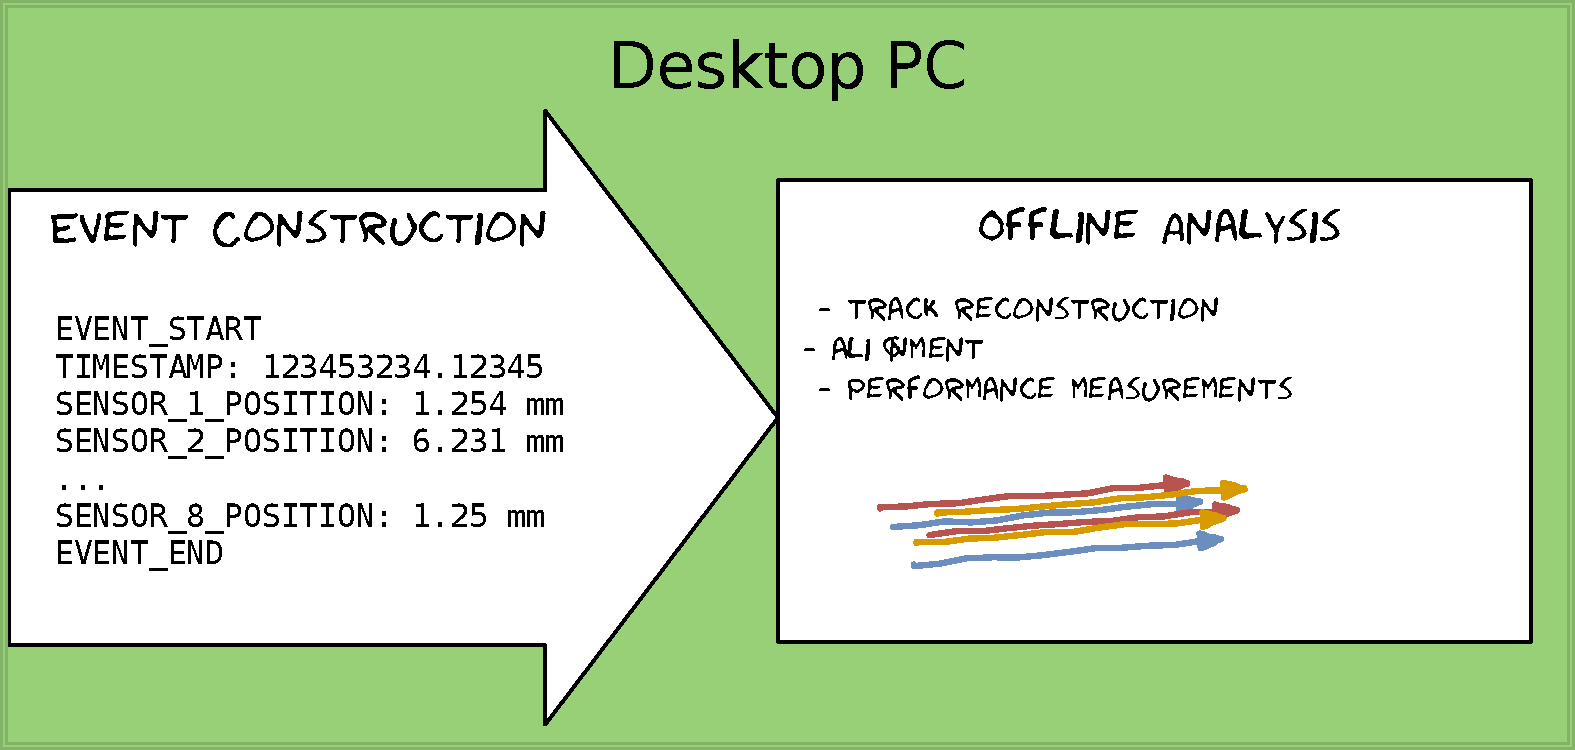
\includegraphics[width=\textwidth]{figures/B3}
\end{figure}
\end{frame}

\section{Firmware}
\begin{frame}{Firmware Architecture}
\begin{figure}
\centering
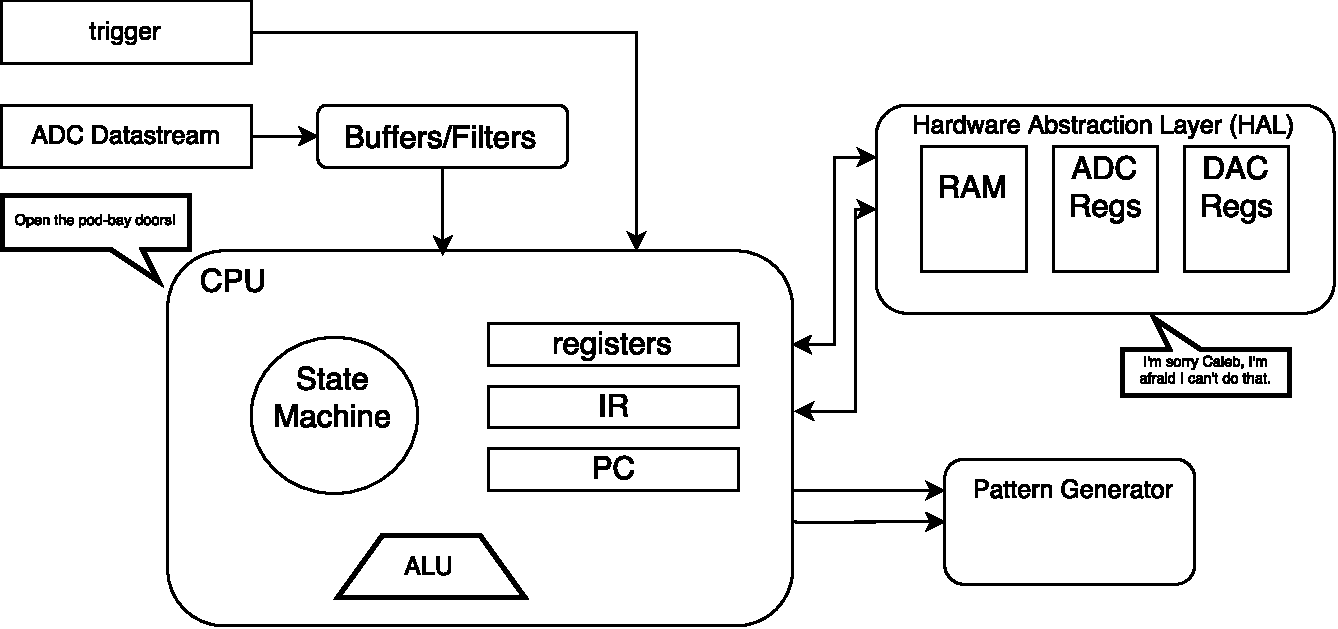
\includegraphics[width=\textwidth]{figures/Firmware_Architecture}
\end{figure}
\end{frame}

\section{Outlook}
\begin{frame}{Outlook}
\checkedbox System design and parts selection \\
\checkedbox APC-128 readout chain proof of concept\\
\checkedbox Circuit design and PCB Layout \\
\checkbox Assembly and offline testing (in progress)\\
\checkbox FPGA Firmware development and testing (in progress) \\
\checkbox Online/Offline software development (in progress) \\
\checkbox Commissioning runs with UNL Diocles electron beam
\end{frame}

\begin{frame}{References}
\textbf{Firmware: } \\
    \small{\url{https://github.com/cfangmeier/VFPIX-telescope-Code/tree/master/DAQ_Firmware}} \\
\textbf{Software: } \\
    \url{https://github.com/cfangmeier/VFPIX-telescope-Code/tree/master/DAQ_Software} \\
\textbf{Hardware: } \\
    \url{https://github.com/cfangmeier/VFPIX-telescope-PCB}\\
\textbf{ICHEP Poster} \\
    \url{https://github.com/cfangmeier/Documents/blob/master/Research/ICHEP_2016_Poster/main.pdf?raw=true}
\end{frame}



\end{document}
